\documentclass[a4paper, 12pt]{article} % Artikel-Klasse

%---------------------------------------------------------
% Encoding, language, quotes
%---------------------------------------------------------
\usepackage[utf8]{inputenc}
\usepackage[ngerman]{babel}       % Deutsche Sprache und Silbentrennung
\usepackage{csquotes}             % Für korrekte Anführungszeichen
\usepackage{listings}
\usepackage{xcolor}

%---------------------------------------------------------
% Graphics & PDF
%---------------------------------------------------------
\usepackage{graphicx}
\usepackage{pdfpages}             % Einbinden von PDF-Seiten
\usepackage{caption}              % Verbesserte Bildunterschriften
\usepackage{subcaption}
\usepackage{comment}


% Customize settings
% Customize settings for a more compact style
\lstset{
    language=Java,                 % Specify Java language for syntax highlighting
    basicstyle=\ttfamily\small,    % Use smaller monospaced font for code
    keywordstyle=\color{blue},     % Style for keywords
    commentstyle=\color{gray},     % Style for comments
    stringstyle=\color{red},       % Style for strings
    numbers=none,                  % No line numbers
    breaklines=true,               % Break long lines
    frame=none,                    % No frame around the code
    xleftmargin=0pt,               % Remove left margin
    xrightmargin=0pt,              % Remove right margin
    aboveskip=5pt,                 % Reduce space above the code block
    belowskip=5pt                  % Reduce space below the code block
}

%---------------------------------------------------------
% Math, units, spacing, etc.
%---------------------------------------------------------
\usepackage{siunitx}
\usepackage{setspace}
\usepackage{textgreek}

% Add float package for "H" float option
\usepackage{float}

%---------------------------------------------------------
% Other packages
%---------------------------------------------------------
\usepackage{ifthen}
\usepackage{acronym}
\PassOptionsToPackage{hyphens}{url} % URLs in Hyperlinks umbrechen
\usepackage[breaklinks=true]{hyperref} 
\usepackage{array}                % Bessere Tabellenformatierung
\usepackage{enumitem}             % Kontrolle über Listen-Layouts
\usepackage{nomencl}
\usepackage{scrlayer-scrpage}     % Header und Footer

% Adjust header and footer heights
\setlength{\headheight}{14.5pt}
\setlength{\footheight}{34.16666pt}

%---------------------------------------------------------
% Bibliography (biblatex mit Biber)
%---------------------------------------------------------
\usepackage[backend=biber, style=numeric]{biblatex}  

\addbibresource{literatur.bib}  

%---------------------------------------------------------
% Platzhalter
%---------------------------------------------------------
\newcommand{\titel}{Umbau und Inbetriebnahme eines Konzeptfahrzeugs zur Erprobung eines neuen Fahrantriebs}
\newcommand{\untertitel}{}
\newcommand{\arbeit}{T3000 Hausarbeit}
\newcommand{\studiengang}{Elektrotechnik}
\newcommand{\studienrichtung}{Fahrzeugelektronik}
\newcommand{\autor}{Luka Tadic}
\newcommand{\abgabe}{14.04.2025}
\newcommand{\bearbeitungszeitraum}{19.01.2025 – 14.04.2025}
\newcommand{\matrikelnr}{5726700}
\newcommand{\kurs}{TFE22–1} % en-dash used here
\newcommand{\firma}{Kramer Werke GmbH}
\newcommand{\betreuerfirma}{Dipl. Ing. (FH) Christian Borgmann}
\newcommand{\gutachterdhbw}{Prof.\ Dr.\ Ing. Konrad Reif}
\newcommand{\jahr}{2025}

%---------------------------------------------------------
% Header und Footer mit Linien
%---------------------------------------------------------
\clearpairofpagestyles{}

% Header with consistent logo placement for two logos and line position
\ohead{%
    \parbox{\textwidth}{% Create a flexible container for both images
        \raisebox{1.5cm}[0pt][0pt]{% Raise the Kramer logo
            
\includegraphics[width=3cm]{images/kramer.png}%
        }%
        \hfill % Horizontal space between the two logos
        \raisebox{1.5cm}[0pt][0pt]{% Raise the DHBW logo
            
\includegraphics[width=3cm]{images/DHBW_d_R_FN_46mm_4c}%
        }%
    }%
    \\[-1.5cm] % Move the header line down
    \rule{\textwidth}{0.4pt} % Horizontal rule for the header line
}


% Footer with consistent alignment and contents below the line
\setkomafont{pagefoot}{\normalfont} % Ensure consistent font style
\cfoot{%
    \rule{\textwidth}{0.4pt}\\ % Horizontal rule
    \vspace{0.3em} % Small vertical space
    \begin{tabular}{@{}p{0.33\textwidth}p{0.33\textwidth}p{0.33\textwidth}@{}}
        \arbeit~& \centering \autor~& \raggedleft~\thepage%
    \end{tabular}
}


\pagestyle{scrheadings}        % Stil aktivieren

%---------------------------------------------------------
% Dokumentbeginn
%---------------------------------------------------------
\begin{document}
\sloppy

%---------------------------------------------------------
% Titelseite
%---------------------------------------------------------
\thispagestyle{empty}  % Kein Header oder Footer auf der Titelseite
\hypersetup{pageanchor=false}

\begin{titlepage}
\enlargethispage{4.0cm}
\sffamily  % Serifenlose Schrift für die Titelseite

% Create a container for both logos at the top
\parbox{0.5\linewidth}{%
    \begin{flushleft}
        
\includegraphics[width=0.4\linewidth]{images/kramer.png}\\[5ex] % Kramer logo on the left
    \end{flushleft}
}
\parbox{0.5\linewidth}{%
    \begin{flushright}
        
\includegraphics[width=0.4\linewidth]{images/DHBW_d_R_FN_46mm_4c}\\[5ex] % DHBW logo on the right
    \end{flushright}
}

% Title and information in the center
\begin{center}

{\fontsize{20.74pt}{24pt}\selectfont
\textbf{\titel}\\[1.5ex]}

{\fontsize{17pt}{20pt}\selectfont
\textbf{\arbeit}\\[2ex]}

{\fontsize{14pt}{17pt}\selectfont
Studiengang \studiengang\\[2ex]}

{\fontsize{12pt}{14pt}\selectfont
Studienrichtung \studienrichtung\\[1ex]
Duale Hochschule Baden-Württemberg Ravensburg, Campus Friedrichshafen\\[5ex]
von\\[1ex]
\autor\\[15ex]}

\end{center}

% Footer-like table with additional information
\begin{center}
{\fontsize{12pt}{14pt}\selectfont
\begin{tabular}{ll}
Abgabedatum:                    & \quad \abgabe\\  
Bearbeitungszeitraum:           & \quad \bearbeitungszeitraum\\  
Matrikelnummer:                 & \quad \matrikelnr\\ 
Kurs:                           & \quad \kurs\\ 
Dualer Partner:                 & \quad \firma\\ % entfällt bei Studienarbeit
Betreuerin / Betreuer:          & \quad \betreuerfirma\\  
Gutachterin / Gutachter:        & \quad \gutachterdhbw\\ [2ex]
\end{tabular}
}
\end{center}

\end{titlepage}

\clearpage

\pagestyle{scrheadings}  % Header und Footer nach Titelseite aktivieren
\hypersetup{pageanchor=true}

%---------------------------------------------------------
% Erklärung
%---------------------------------------------------------

\pagenumbering{Roman}

\section*{Erklärung}
\begin{spacing}{1.8}  % Adjust line spacing
    \fontsize{14pt}{14pt}\selectfont

Ich versichere hiermit, dass ich meine \arbeit\ mit dem Thema:

\begin{quote}
    \textit{\titel}
\end{quote}

selbstständig verfasst und keine anderen als die angegebenen Quellen und Hilfsmittel benutzt habe.  
Ich versichere zudem, dass die eingereichte elektronische Fassung mit der gedruckten Fassung übereinstimmt.\\[6ex]

Friedrichshafen, den \today \\[1ex]
\rule[-0.2cm]{5cm}{0.5pt} \\  
\autor\\[10ex]

\rmfamily

\end{spacing}
\clearpage

\section*{Kurzfassung}
\begin{spacing}{1.8}  % Adjust line spacing
    \fontsize{14pt}{14pt}\selectfont  % Font size and line spacing
    Im Rahmen dieses Projekts wird ein \acf{PoC}-Umbau an einem Kramer 415–38 Fahrzeug durchgeführt,
    um die Praxistauglichkeit eines neuen Fahrantriebskonzepts zu überprüfen. Ziel ist es, die Leistung,
    Dynamik und Reststeigfähigkeit des Fahrzeugs zu verbessern sowie Geräuschreduzierung und Kraftstoffverbrauch zu reduzieren.
    
    Der Umbau umfasst die Integration neuer Komponenten, darunter der Danfoss \ac{BPC}-Fahrantrieb,
    eine Servobremse, das Rafi Gen2 Display sowie der Einbau der neuen Keypads
    mit unterschiedlichen Fahrmodi-Optionen. Die Umsetzung beinhaltet mechanische Anpassungen sowie die
    Softwareintegration des neuen Systems. Nach dem Einbau wird das Fahrzeug getestet, um zu evaluieren,
    ob die gewünschten Effekte erreicht wurden.
    
    Das Projekt soll zeigen, ob sich das neue Fahrantriebskonzept erfolgreich in die T07/T08-Fahrzeugreihe
    integrieren lässt und somit die Wettbewerbsfähigkeit der Kramer Telelader steigert.
    
\end{spacing}

\clearpage
%---------------------------------------------------------
% Abstract
%---------------------------------------------------------
\section*{Abstract}
\begin{spacing}{1.8}  % Adjust line spacing
    \fontsize{14pt}{14pt}\selectfont  % Font size and line spacing
    As part of this project, a \acf{PoC} conversion will be carried out on a Kramer 415–38 vehicle
to evaluate the practicality of a new drive system concept. The goal is to improve the vehicle’s
performance, dynamics, and residual climbing ability, as well as to reduce noise and fuel consumption.

The conversion includes the integration of new components, such as the Danfoss \ac{BPC} drive system,
a servo brake, the Rafi Gen2 display, and the installation of new keypads
with various driving mode options. The implementation involves mechanical modifications as well as
software integration of the new system. After installation, the vehicle will be tested to assess
whether the desired effects have been achieved.

The project aims to demonstrate whether the new drive concept can be successfully integrated
into the T07/T08 vehicle series, thereby enhancing the competitiveness of the Kramer telehandlers.


\end{spacing}
\clearpage

% List of figures
%\listoffigures

\section*{Abkürzungsverzeichnis}
\begin{spacing}{1.8}  % Adjust line spacing
    \fontsize{14pt}{14pt}\selectfont  % Font size and line spacing

\begin{acronym}
    \acro{PoC}{Proof of Concept}
    \acro{BPC}{Best Point Control}
    \acro{CAN}{Controller Area Network}
\end{acronym}

\end{spacing}

\clearpage
\begin{spacing}{1.5}  % Adjust line spacing
    \fontsize{14pt}{14pt}\selectfont  % Font size and line spacing

%---------------------------------------------------------
% Inhaltsverzeichnis
%---------------------------------------------------------
\tableofcontents

\end{spacing}

\clearpage
\pagenumbering{arabic}


\section{Einleitung und Motivation}
\begin{spacing}{1.5}  % Adjust line spacing
\fontsize{14pt}{14pt}\selectfont  % Font size and line spacing
Im Rahmen dieses \acf{PoC}-Umbaus wird untersucht, ob das 
geplante Fahrantriebskonzept für die T07/T08-Modelle der Kramer-Telelader 
die gewünschten Verbesserungen hinsichtlich Leistung, Dynamik und 
Reststeigfähigkeit erzielt. Ziel des Projekts ist es, die Wettbewerbsfähigkeit
der Fahrzeuge weiter zu steigern, indem innovative Technologien und 
Optimierungsmaßnahmen implementiert werden.

Der Ausgangspunkt für diese Entwicklung waren die Ergebnisse des
„Voice of Sales/Voice of Engineering“-Events im Juli 2021, bei dem 
spezifische Anforderungen an den Fahrantrieb definiert wurden. 
Wesentliche Optimierungen umfassen die Einführung des Danfoss 
\acf{BPC}-Fahrantriebs, der trotz der erzielten Kostenreduzierung eine höhere 
Leistung sowie ein erhöhtes Drehmoment ermöglicht. Zudem werden Maßnahmen 
wie die stärkere Absenkung der Dieseldrehzahl auf 1800 U/min zur Reduzierung
von Geräuschen und Kraftstoffverbrauch sowie die Implementierung 
unterschiedlicher Fahrmodi berücksichtigt.

Zur Risikominimierung kommt die Best Point Software zum 
Einsatz, während durch das neue Servo-Bremskonzept sowohl die Fahrsicherheit 
als auch der Bedienkomfort verbessert werden. Ergänzend trägt die Einführung 
von AMA-Keypads zur weiteren Kostenreduzierung als auch zur Verwendung 
verschiedener Fahrmodi bei.

Diese Arbeit analysiert die technischen 
Anpassungen und bewertet deren Auswirkungen auf die 
Gesamtperformance des Fahrantriebssystems.

\end{spacing}

\section{Zielsetzung}
\begin{spacing}{1.5}  % Adjust line spacing
    \fontsize{14pt}{14pt}\selectfont  % Font size and line spacing

    Ziel dieses Projekts ist die Umsetzung eines \ac{PoC}-Umbaus 
    am Fahrzeugtyp 415–38 durch Integration und Inbetriebnahme 
    eines neuen Fahrantriebskonzepts.
    
    Für den Projekterfolg sind zwei Kernbereiche entscheidend:
    
    \textbf{1. Fahrzeugumbau:}
    Der Umbau zielt auf die fachgerechte Implementierung des neuen Antriebssystems ab. 
    Wichtige Punkte dabei sind:
    
    \begin{itemize}
        \item Schutz der Komponenten
        \item Optimale Positionierung und Integration
        \item Elektrische und mechanische Kompatibilität
        \item Sorgfältige Dokumentation
    \end{itemize}
    
    \textbf{2. Inbetriebnahme und Prüfung:}
    Im Anschluss wird das System getestet, um folgende Aspekte zu validieren:
    
    \begin{itemize}
        \item Erfolgreiche Senkung der Dieseldrehzahl
        \item Messbare Geräusch- und Verbrauchsreduktion
        \item Erfüllung der Anforderungen an Leistung und Dynamik
        \item Funktion der neuen Komponenten (z.B. Keypad-Funktionen, Rafi Gen2 Display)
    \end{itemize}
    
    Die strukturierte Umsetzung soll sicherstellen, 
    dass das Konzept die gewünschten Verbesserungen liefert.
    
\end{spacing}

\section{Ablauf Umbau und Inbetriebnahme}
\begin{spacing}{1.5}
\fontsize{14pt}{14pt}\selectfont

Der Umbau und die Inbetriebnahme des Fahrzeugs erfolgten in mehreren aufeinander abgestimmten Schritten. 
Dieses Kapitel beschreibt die wesentlichen Phasen des Umbaus sowie die durchgeführten 
Maßnahmen zur erfolgreichen Implementierung des neuen Fahrantriebskonzepts.

\subsection{Umbau des Fahrzeugs}
Der Umbau umfasste verschiedene mechanische und elektrische Anpassungen zur Integration der neuen Komponenten. Die Arbeiten konzentrierten sich auf folgende Punkte:

\begin{itemize}
    \item \textbf{Hardwareanpassungen:} Die Keypads wurden in das Fahrzeug integriert, indem bereits vorhandene Kabelstränge wie die Versorgungsspannung und \ac{CAN}-Bus-Signale von bestehenden Komponenten wie dem Radio oder dem Joystick abgesplicet und an die Keypads weitergeführt wurden. Auch das Rafi Gen2 Display wurde auf diese Weise elektrisch eingebunden.
    
    \begin{figure}[H]
        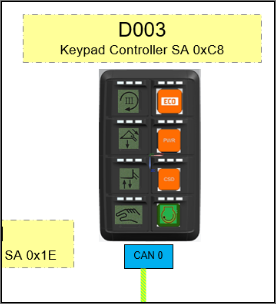
\includegraphics[width=0.4\linewidth]{images/Keypad Foto.png}\\[1ex]
        \centering
        \caption{Ausschnitt aus Systemschaltbild vom Keypad aus dem PoC-Projekt}
        \label{ABBILDUNG}
    \end{figure}

    \begin{figure}[H]
        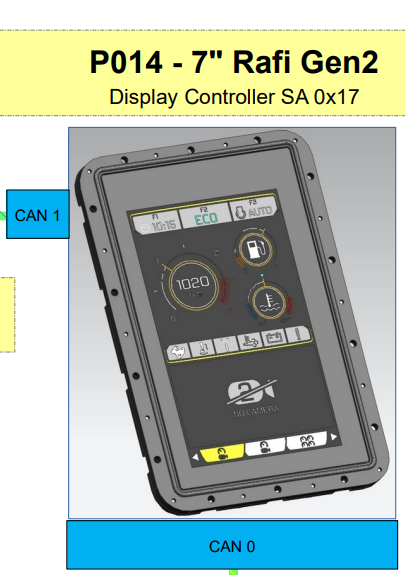
\includegraphics[width=0.4\linewidth]{images/Display.png}\\[1ex]
        \centering
        \caption{Ausschnitt aus Systemschaltbild vom Display aus dem PoC-Projekt}
        \label{ABBILDUNG}
    \end{figure}

    \item \textbf{Montage neuer Komponenten:} Die neuen Bauteile wurden gemäß den technischen Vorgaben installiert und elektrisch angeschlossen. Dabei wurde besonderes Augenmerk auf die korrekte Pin-Belegung (Pinning) sowie die sichere Befestigung der Komponenten im Fahrzeug gelegt.
    
    \item \textbf{Integration ins System:} Der BPC-Controller wurde gemäß der bereitgestellten Dokumentation vorbereitet und gepinnt. Der finale Anschluss erfolgte nach dem Einbau der neuen Fahrpumpe. Anschließend wurden die vorbereiteten Leitungen mit den bereits vorhandenen Komponenten wie Handgas, Sitzkontaktschalter und \ac{CAN}-Bus verbunden, um eine vollständige Integration ins bestehende Fahrzeugsystem zu gewährleisten.
\end{itemize}

Zur Vorbereitung des Umbaus wurde ein detailliertes Systemschaltbild mit Microsoft Visio erstellt.

\begin{figure}[H]
    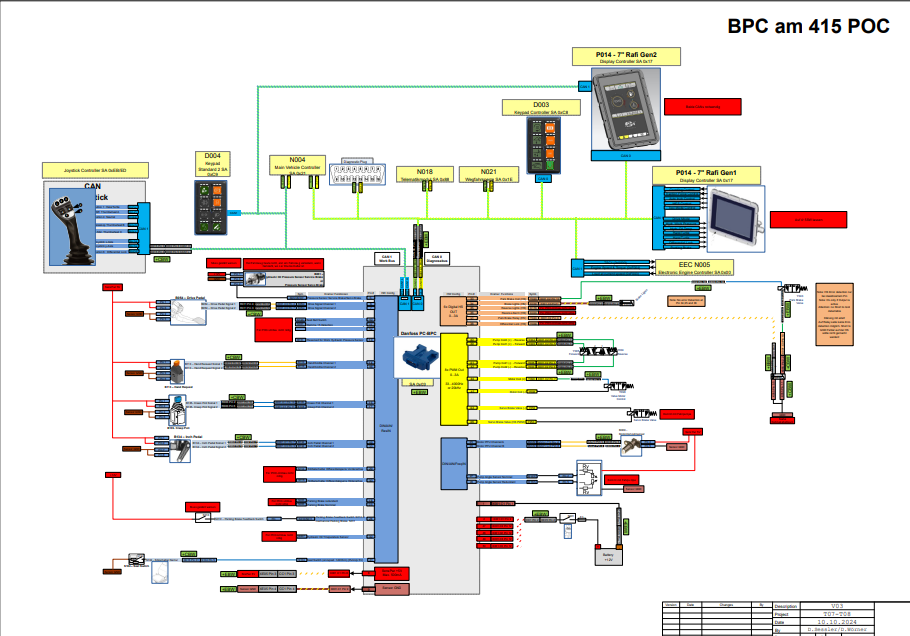
\includegraphics[width=0.9\linewidth]{images/Systemschaltbild.png}\\[1ex]
    \centering
    \caption{Systemschaltbild des Fahrzeugs}    
    \label{ABBILDUNG}
\end{figure}

Es diente als Grundlage für die elektrische Integration und zeigt die Zusammenhänge zwischen den neuen Komponenten. In den folgenden Abbildungen sind exemplarische Ausschnitte des BPC-Controllers und eines Keypads dargestellt. Die Verbindung und Funktion der Keypads wurden entsprechend dem Systemschaltbild umgesetzt. Eine schematische Darstellung dazu findet sich in der  folgenden Abbildung:

\begin{figure}[H]
    
\includegraphics[width=1\linewidth]{images/Keypads Mindmap.png}\\[1ex]
    \centering
    \caption{Modelldarstellung: Funktionen und Anschlussschema des Keypads}
    \label{ABBILDUNG}
\end{figure}

Ein zentrales Element des Umbaus war die Integration der neuen Keypads. Diese wurden nicht nur zur Kostenreduktion, sondern auch zur Erweiterung der Fahrzeugfunktionen eingesetzt. Die Tasten ermöglichen die Aktivierung verschiedener Fahrmodi und Funktionen, darunter:

\begin{itemize}
    \item \textbf{Feststellbremse/Parkbremse:} Aktivierung oder Lösung der Bremse mit Statusanzeige über Funktionsbeleuchtung. Zum Lösen ist ein gewisser Pedalweg über das Inchpedal erforderlich.
    
    \item \textbf{Schaufelmodus:} Ermöglicht beim Absenken des Hubarms eine proportionale Mitsteuerung des Einzugs.
    
    \item \textbf{ECO-Modus:} Anpassung der Motordrehzahl an den Leistungsbedarf von Arbeitshydraulik und Fahrpedal.
    
    \item \textbf{Power-Modus:} Erhöhung der Motordrehzahl in Abhängigkeit zur Gaspedalstellung.
    
    \item \textbf{Constant Speed Drive:} Aktiviert die Langsamfahreinrichtung.
    
\end{itemize}

Neben diesen Funktionen gibt es noch weitere Optionen auf den Keypads, die die Bedienung und Kontrolle des Fahrzeugs weiter erleichtern. Diese werden ebenfalls durch den BPC-Controller gesteuert und sind integrale Bestandteile der neuen Fahrzeugbedienlogik.


 \subsection{Installation der BPC-Software}
 Nach dem mechanischen Umbau soll die \acs{BPC}-Software auf dem entsprechenden Controller installiert werden.
 Dies erfordert sowohl hardwareseitige Anpassungen als auch softwaretechnische Konfigurationen, die im Rahmen der Umsetzung erfolgen.
 Die korrekte Pin-Belegung (Pinning) wird mithilfe relevanter Dokumentation überprüft und dokumentiert.
 

 \subsection{Inbetriebnahme}
 Nach der Installation und Validierung der neuen \acs{BPC}-Software soll das Fahrzeug in Betrieb genommen und getestet werden. Dabei wird überprüft, 
 ob die Erwartungen an den neuen Fahrantrieb im \acs{PoC}-Fahrzeug erfüllt werden.
 
 Im Rahmen der Tests sollen alle relevanten Parameter kontrolliert und 
 die Funktionalität der neu integrierten Komponenten sichergestellt werden. 
 
 Durch die Inbetriebnahme soll festgestellt werden, 
 ob die geplanten Optimierungen erfolgreich umgesetzt wurden und das Fahrantriebskonzept mithilfe des BPC-Controllers und der Software die gewünschten Verbesserungen erzielt.
 
 
\end{spacing}

\section{Ergebnisse und Ausblick}
\begin{spacing}{1.5}  % Adjust line spacing
    \fontsize{14pt}{14pt}\selectfont  % Font size and line spacing

    Im Verlauf des Projekts wurden wertvolle Erkenntnisse gewonnen, die als Grundlage für künftige Weiterentwicklungen dienen. Der \acf{PoC}-Umbau hat gezeigt, welche Optimierungen am Fahrantriebskonzept erfolgreich waren und welche Aspekte weiter verbessert werden müssen.

    Alle erforderlichen Kabel und Komponenten wurden beschafft, abgemessen, gepinnt und für den Einbau vorkonfektioniert. Die Keypads und das Rafi Gen2 Display konnten erfolgreich angeschlossen werden und sind bereit für den Einsatz. Die neue Fahrpumpe konnte jedoch aufgrund des begrenzten Zeitrahmens noch nicht eingebaut werden, sodass der Umbau nur teilweise abgeschlossen ist.

    Trotz dieser Einschränkungen wurden viele wertvolle Erkenntnisse gewonnen, insbesondere in der Dokumentation der Ergebnisse, der Nutzung von Microsoft Visio zur Erstellung von Systemschaltbildern und der korrekten Verkabelung der Fahrzeugkomponenten.

    Nach Abschluss der Phase wird der Umbau des Hydraulik-\acs{PoC} fortgesetzt, gefolgt von der Beschaffung und Vorbereitung des ersten Prototypen. Die Erfahrungen aus diesem \acs{PoC} fließen direkt in die nächste Entwicklungsstufe ein, um die Effizienz des Fahrantriebs weiter zu optimieren.

    Langfristig soll das Projekt dazu beitragen, die Wettbewerbsfähigkeit der Kramer Telelader durch innovative Technologien zu steigern und die Effizienz der Fahrzeuge nachhaltig zu verbessern.
\end{spacing}



\clearpage

%---------------------------------------------------------
% Bibliografie
%---------------------------------------------------------
\begingroup
\renewcommand{\bibfont}{\fontsize{13pt}{12pt}\selectfont}  
\sloppy
\nocite{*}
\begin{spacing}{1.5}  % Adjust line spacing
\fontsize{14pt}{14pt}\selectfont  % Font size and line spacing
\printbibliography{}
\end{spacing}
\end{document}
